\chapter{Testy środowiska symulacyjnego}
\label{sec:tests}
W tym rozdziale przedstawione są różne konfiguracje pakietów, wraz z wykresami ruchów platform, oraz wnioski płynące z tych zachowań.
Każdy test wymaga innego podłączenia pakietów do siebie nawzajem.

Wyniki pomiarów zostały zebrane za pomocą ROSowego narzędzia \texttt{rosbag}, a następnie wyeksportowane do pliku CSV. Za pomocą programu Gnuplot narysowano wykresy.

\section{Testy enkoderów}
	Model czujnika enkoderów zwraca aktualną prędkość i pozycję kół modelu dynamicznego.
	W ten sposób jest możliwe dokładniejsze określenie pozycji platformy, niż bazując na modelu kinematycznym.
	Jednakże, ta metoda także ma swoje ograniczenia, ze względu na poślizgi, zatem program sterujący nie może w pełni bazować na tych czujnikach, a jedynie powinien używać ich pomocniczo.
	
	W tym teście obliczono pozycję modelu kinematyki, bazując na danych zebranych przez modele enkoderów.
	W najlepszym przypadku, pozycje powinny być identyczne.
	
	\begin{figure}[H]
		\centering
		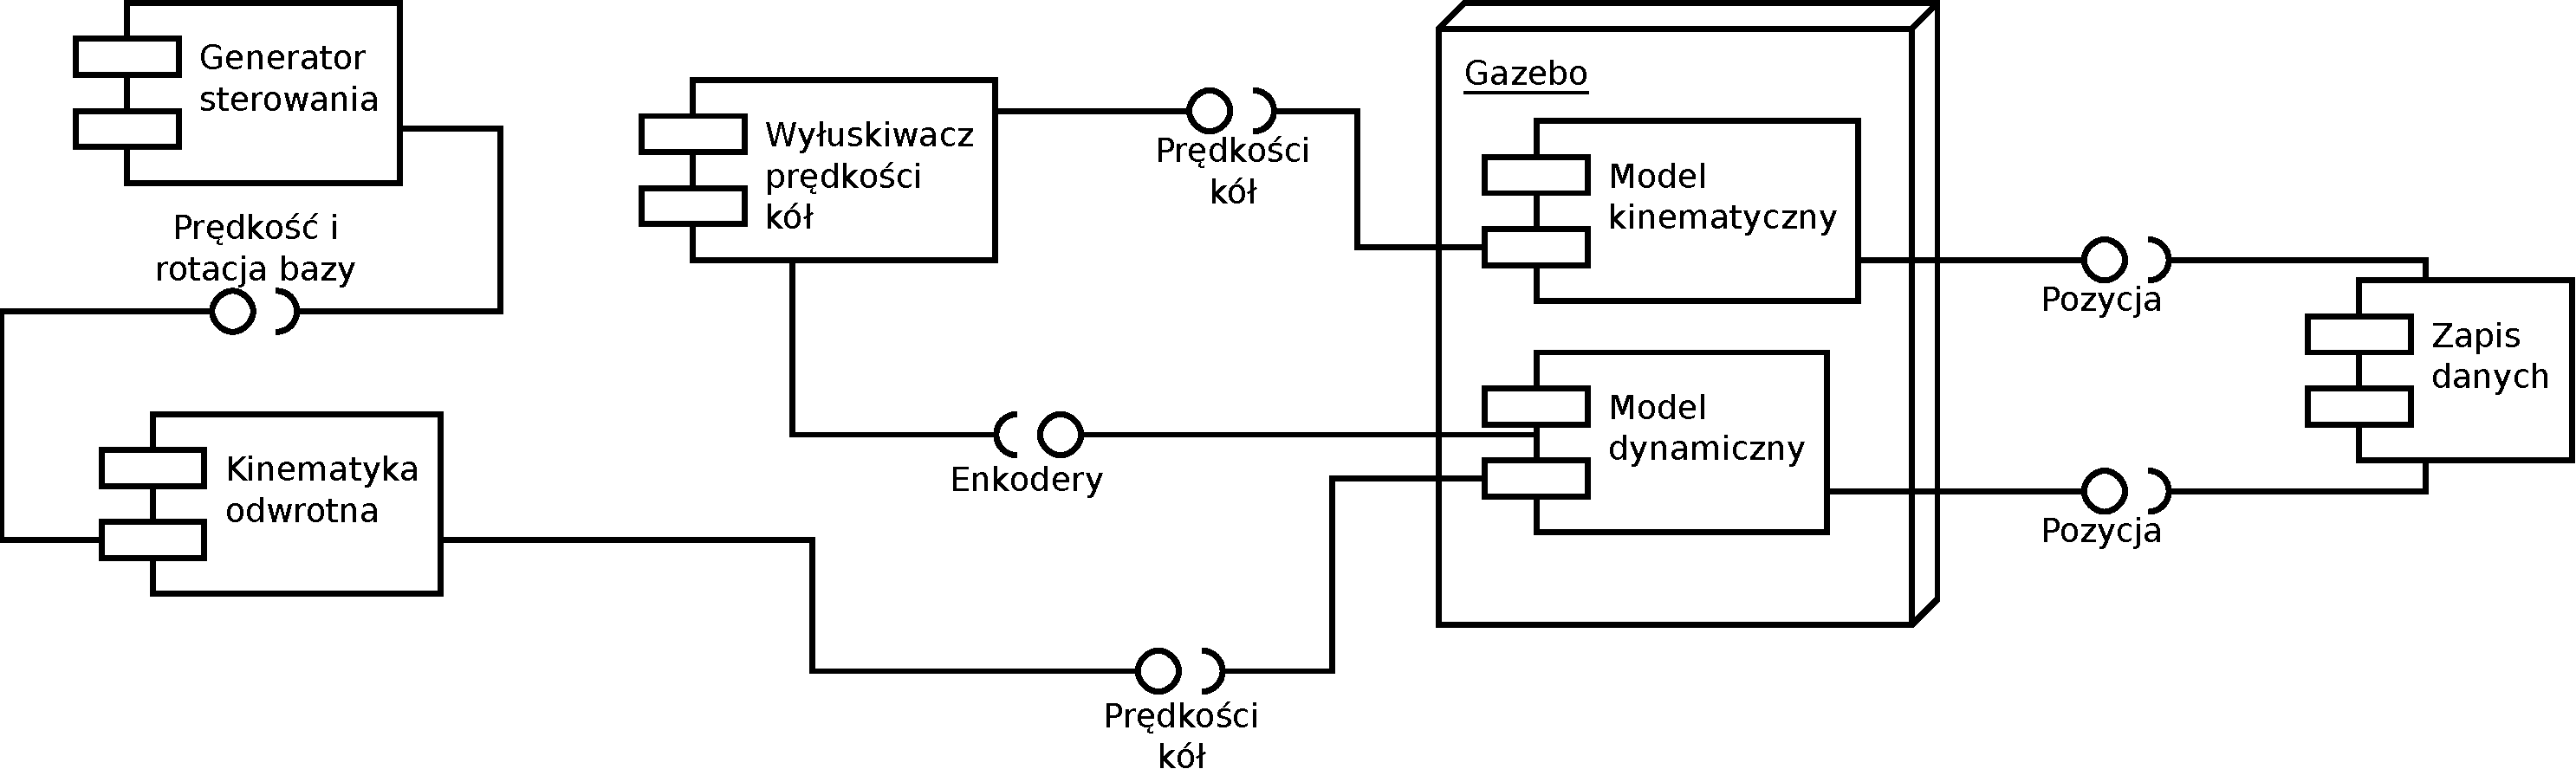
\includegraphics[width=\textwidth]{uml/encoders.pdf}
			\caption{Połączenie komponentów w celu sprawdzenia poprawności działania enkoderów modelu dynamicznego.}
		\label{plot:encoders}
	\end{figure}
	
	Wyjście enkoderów modelu dynamicznego wyłuskane jest z wiadomości i podane dla modelu kinematycznego, model platformy kinematycznej porusza się tak, jak odbiera to model platformy dynamicznej. 
	
	Przeprowadzono dwa testy, w pierwszym nadawano prędkości kołom z odpowiednią częstotliwością, drugi nadawał prędkości kół jedynie przy zmianie kierunku ruchu modelu dynamicznego.
	Sterowanie zostało stworzone z myślą o wywołaniu poślizgów platformy, nadana prędkość 0,5 $\frac{m}{s}$ była większa, niż w poprzednich testach.
	
	\begin{figure}[H]
		\centering
		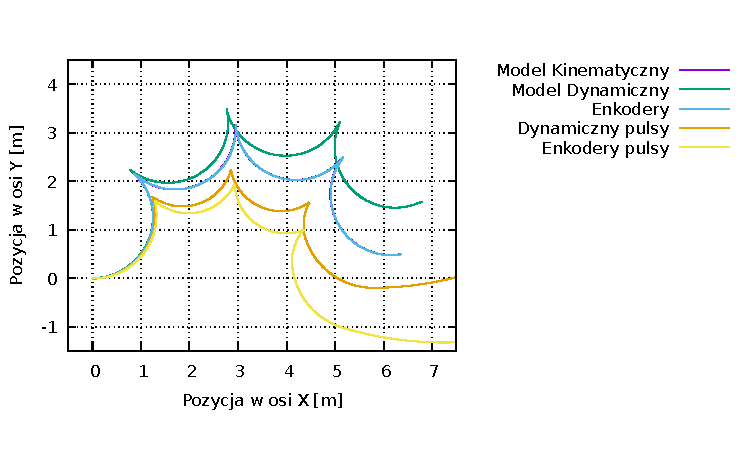
\includegraphics[width=\textwidth]{plots/star_encoders.pdf}
			\caption{Ruch modeli przy ciągłym wysyłaniu pakietów, jedynie na zmiany kierunku i kinematyka bazująca na danych zebranych z enkoderów. Wykres pierwszy i trzeci są na siebie nałożone.}
		\label{plot:star_encoders}
	\end{figure}
	
	\subsection{Ciągłe nadawanie prędkości kół}
		Przy ciągłym nadawaniu prędkości kołom, enkodery odczytują praktycznie dokładnie te same wartości, jakie są nadawane.
		Co za tym idzie, działa to w taki sam sposób, w jaki działałaby platforma kinematyczna w poprzednim teście.
		Pierwsze trzy wykresy zatem nie różnią się przebiegiem, niż gdyby je wygenerować w poprzednim podłączeniu komponentów.
		
		Przy pierwszej zmianie prędkości platformy, widać różnicę w pozycji modeli, spowodowaną poślizgiem.
		Duża prędkość kątowa również powoduje poślizg kątowy, przez co różnica pomiędzy pozycjami w tym samym czasie rośnie szybciej, jak w poprzednich testach.
		Enkodery nie są w stanie wykrywać poślizgu, dlatego ich wykres nie odstaje w momentach zmiany kierunku od wykresu modelu kinematycznego.
		
	\subsection{Impulsowe nadawanie prędkości kół}
		Jedno wywołanie metody maszyny symulacyjnej fizyki nadaje prędkość kołom. Następnie, z powodu symulowanych oporów, prędkość koła naturalnie spada, aż do
		ponownego nadania prędkości. To, jak prędkość ruchu spada, widać, gdyż segmenty przebiegu w dwóch ostatnich wykresach nie są łukami, jak ma to miejsce przy 
		ciągłym nadawaniu prędkości. Po nadaniu ostatniej wiadomości, zatrzymującej wszystkie koła, platforma nadal wolno się porusza, pod wpływem bezwładności, a brak oporu rolek w jednym z kierunków, oraz brak oporu obrotu koła pozwalał na ciągły ruch w losowym kierunku.
		
		Co warto tutaj zauważyć, to to że enkodery prawidłowo starają się przekazać zmienną prędkość kół. 
		Inaczej mówiąc, pozycja wynikająca z danych zwróconych z enkoderów jest dokładniejsza, niż wynikająca z wywołanego ruchu modelu kinematycznego w idealnym przypadku.
		Żółty wykres jest bliżej pomarańczowego, niż fioletowy/niebieski.
		Tutaj także widać wpływ poślizgu modelu na określanie pozycji.
		
		Zatem model enkoderów może mieć faktyczne zastosowanie w określaniu pozycji platformy. 
		Okazuje się lepszy, niż kinematyka, w przypadku zewnętrznego nadania prędkości platformie, na przykład pod wpływem nagłego zatrzymania.
		Pod warunkiem, że nie występuje poślizg. Jak już wcześniej wspomniano, platforma jest podatna na ruch w losowym kierunku przy nagłym zatrzymaniu,
		lecz nie zawsze taki ruch może zostać niewykryty. Poślizg, a nadanie niedeterministycznej siły zewnętrznej, to dwa różne zjawiska.
		

\section{Ruch platformy po kwadracie}
	Za pomocą pakietu nadającego sterowanie z pliku, opisanego w sekcji \ref{sec:gramofon}, podano robotowi i platformie proste sterowanie.
	Ruch odbywał się przez 10 \si{\second} z prędkością 0,1 \si{\metre\per\second} na dystansie 1 \si{\metre}, kolejno w kierunkach -X, -Y, X i Y.
	Zmiana kierunku prędkości odbywała się natychmiastowo, powodując poślizgi.
	W tym teście nie nadawano prędkości kątowej.
	
	Pozycja modelu została łatwo wygenerowana, ponieważ symulacja odbywała się w przestrzeni wirtualnej.
	Pozycja platformy nie mogła być łatwo określona. Posłużono się algorytmem ROSowego pakietu \texttt{laser_scan_matcher}, który na podstawie 
	danych z jednego i drugiego skanera laserowego określił aktualną pozycję platformy. Określenie pozycji jest obarczone błędem wynikającym
	z błędów pomiarowych czujników, stąd obliczona trasa nie składa się z odcinków.
	
	
	
\section{Jednostka inercyjna}
\label{sec:test_imu}
	Test polega na wymuszeniu określonych prędkości i przyspieszeń na modelu bazy i zebraniu wyników.
	
	\begin{figure}[H]
		\centering
		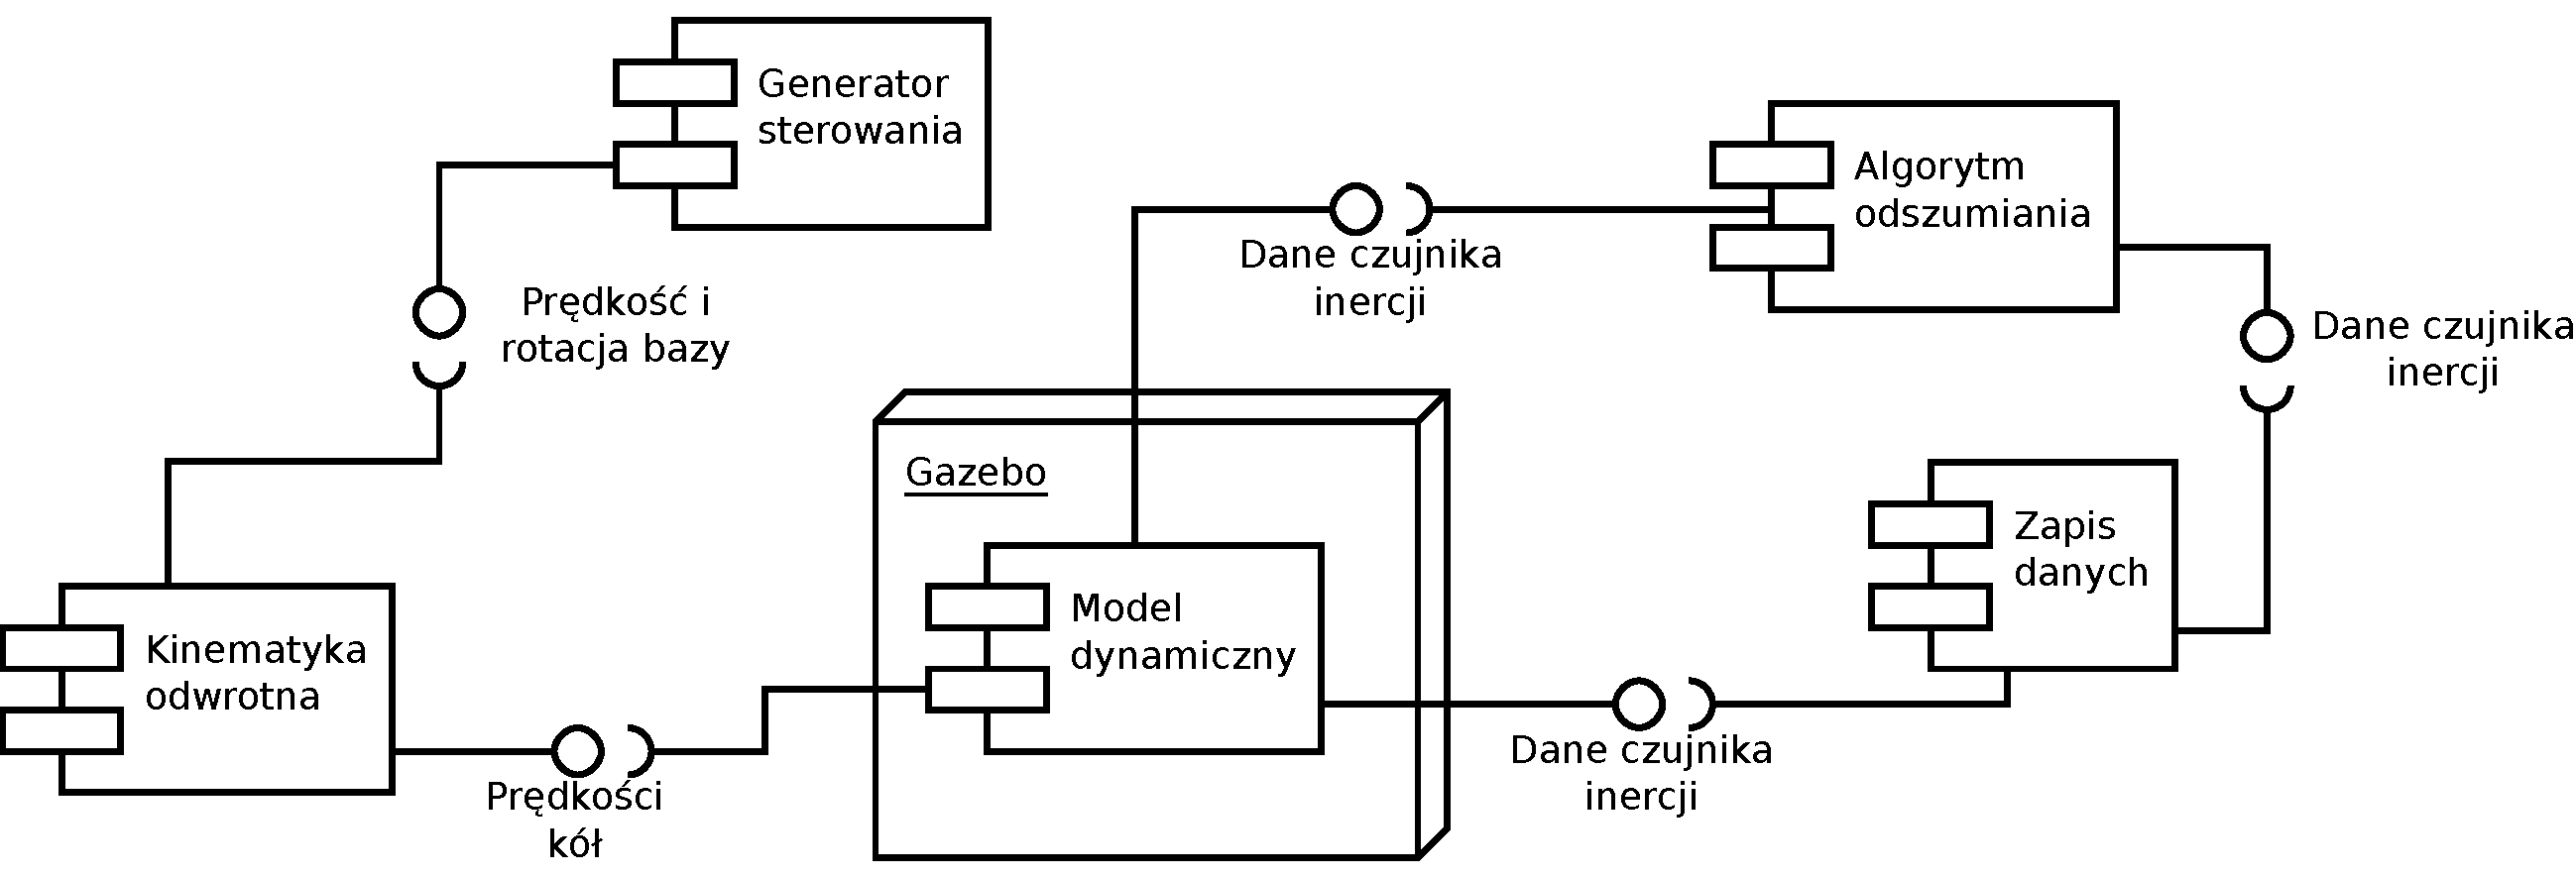
\includegraphics[width=\textwidth]{uml/wewucho.pdf}
		\caption{Połączenie komponentów dla testu czujnika inercji.}
		\label{uml:wewucho}
	\end{figure}
	
	Połączenie nadające sterowanie jest podobne do poprzednich testów.
	Dodatkowy komponent odszumia dane i zapisuje je, aby można je było wygodnie przedstawić na wykresie.
	W tym teście nie jest wymagany model kinematyczny.
	
	\subsection{Czujnik prędkości kątowej}
		Ten czujnik korzysta z żyroskopu i zwraca prędkość kątową we wszystkich trzech osiach.
		Ponieważ jednak platforma porusza się po płaskim terenie, wymagany jest jedynie czujnik w kierunku osi Z, czyli w górę.
		Drugą osią może być zatem czas nadania pakietu.
		
		Wykonano dwa testy, w pierwszym wymuszono ruch po spirali ze stałą prędkością liniową, a co za tym idzie, z nieliniowo zmieniającą się prędkością kątową platformy.
		Prędkość platformy aktualizowana była co 0,5 s, co widać w postaci schodków na wykresie.
		Trasa robota nie pokazywała żadnych nowych zjawisk, które nie zostały już wspomniane w poprzednich testach.
		
		Drugim testem jest ruch po serpentynie.
		Prędkość liniowa platformy była stała, nadawano prędkości kątowe o rosnącej wartości. Model jeździł po łukach o coraz mniejszych promieniach.
		
		Testy rozpoczęły się w tym samym czasie, lecz program nadający sterowanie celowo oczekiwał po rozpoczęciu kilka sekund.
		
		\begin{figure}[H]
		\centering
			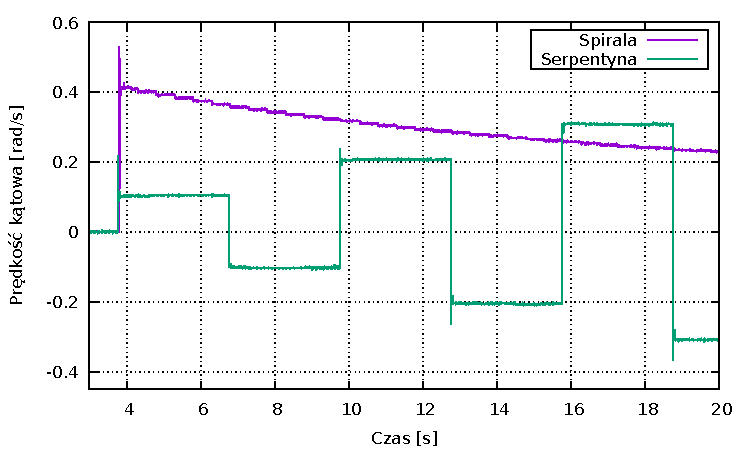
\includegraphics[width=\textwidth]{plots/wewucho_angular.pdf}
			\caption{Test prędkości kątowej czujnika inercji.}
			\label{plot:wewucho_angular}
		\end{figure}
		

		Na początku generowany jest szpikulec, przy natychmiastowym nadaniu prędkości kątowej i liniowej platformie.
		Jest to wewnętrzny szum generowany przez maszynę symulacyjną fizyki, spowodowany dużą zmianą wielu jej parametrów.
		Również wszystkie składowe elementy modelu są symulowane oddzielnie, połączone razem za pomocą więzów.
		Zatem informacja nadająca prędkość platformie przechodzi przez kilka warstw, zanim ustawi odpowiednie prędkości wszystkim składowym systemu.
		
		Widać także niewielką sprężystość modelu, objawia się ona chwilowym zmniejszeniem wartości wielkości tuż po szpikulcu.
		Nie jest to celowo zasymulowana mechanika, a naturalne zjawisko reakcji na akcję. Jeden element składowy platformy działa na drugi, ale za chwilę drugi element także
		zaczyna działać na pierwszy. Podobne jest to w działaniu przeregulowania regulatora.
		
		Jest to zachowanie zbliżone do odczytów z jednostki inercji robota. Tam czujnik również zwraca takie nagłe skoki prędkości w trakcie ruchów.
		Szum w trakcie jednostajnego obrotu jest bardzo podobny.
		
	\subsection{Czujnik przyspieszenia liniowego}
		Jak wcześniej wspomniano, maszyna do symulacji nie posiada wewnętrznie informacji o przyspieszeniu obiektu, gdyż działa w dyskretnych przedziałach czasowych.
		Wartość przyspieszenia musi zostać celowo obliczona, co powodować może różne błędy.
		
		W tym teście platformie nadano przyspieszenie 2 $\frac{m}{s^2}$ przez czas 1 s, w kierunku osi X, w wiadomościach co 0,1 s.
		Następnie platforma poruszała się przez 5 s z prędkością 0,2 $\frac{m}{s}$.
		Potem nadano jej jednoczesne opóźnienie w kierunku osi X i przyspieszenie w kierunku Y, o tych samych wartościach, co na początku.
		Po kolejnych 5 s, platforma zwolniła do zera. Kształt trasy przypominał literę L z zaokrąglonym kątem.
		Samo przyspieszenie platformy wynika z uśrednienia wysyłanych prędkości w czasie, musi być nadawane dyskretnie, żaden z elementów symulatora nie jest w stanie
		pracować w ciągłej domenie czasowej.
		
		\begin{figure}[H]
		\centering
			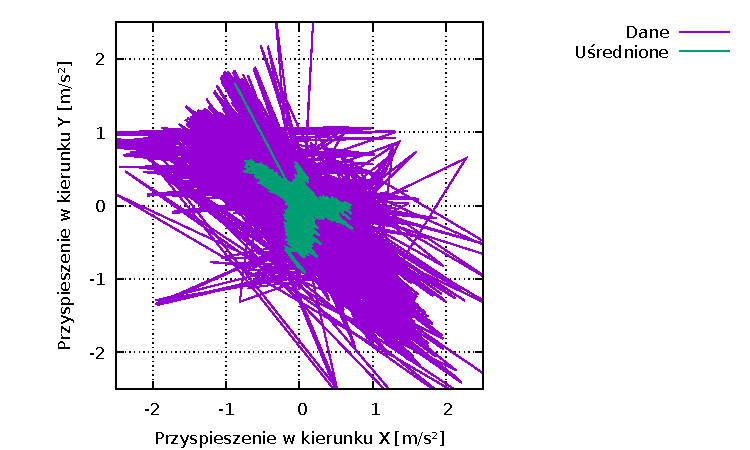
\includegraphics[width=\textwidth]{plots/wewucho_linear.pdf}
			\caption{Test przyspieszenia czujnika inercji.}
			\label{plot:wewucho_angular}
		\end{figure}
		
		Na czystych danych nie widać, jakoby model czujnika inercji w ogóle działał. 
		Jest to widoczne tylko przy natychmiastowej zmianie prędkości platformy, to jest przy teście \ref{sec:test_square}.
		Jednak takie teoretycznie nieskończone przyspieszenie nie może być w żaden naukowy sposób zinterpretowane, dlatego należy przeprowadzić testy z kontrolowanym
		przyspieszeniem.
		
		Po uśrednieniu danych z 10 ostatnich pomiarów, okazuje się, że środek generowanych w tym czasie danych jednak się przesuwał.
		Co więcej, robił to w poprawnych kierunkach.
		
		Na początku powstał zapis w kierunku dodatnim osi X, reprezentujący przyspieszenie platformy.
		Następnie program zanotował odchylenie pod kątem 45°, w drugiej kwadrze, co było nałożeniem się opóźnienia w osi X i przyspieszenia w osi Y.
		Na koniec zatrzymanie się platformy generowało zapis w ujemnym kierunku osi Y.
		
		Wykres generowany w czasie rzeczywistym sugeruje, jakoby niektóre pakiety przekazywały zerowe przyspieszenie, co w znaczącym stopniu wpływa na 
		ostatecznie generowane dane.
		
		Widać także, że wyraźnie zapisuje się tendencja danych do oscylowania na prostej pod kątem 45°.
		
		Akcelerometr platformy generuje bardzo podobne dane, które również są obarczone dużym błędem.
		Można powiedzieć zatem, że symulacja czujnika jest na dobrym poziomie.
		
		
		
		
		
	
	
